%Preambulo
\documentclass{article}
\usepackage[spanish]{babel}
\usepackage[utf8]{inputenc}
\usepackage{graphicx}
\usepackage{float}
\usepackage{subfig}
\usepackage{xcolor}
\usepackage{hyperref}
\title{\textbf{El tiro parabólico}}
\date{Mecánica Newtoniana. Prácticas de ordenador. Grupo 1. Grado en Física. Curso 2022-23}
\author{Aroa Antón Samaniego}

%Cuerpo
\begin{document}

\definecolor{w}{rgb}{255,255,255}
\hypersetup{linkbordercolor={w},urlbordercolor={w},citebordercolor={0 0 0}}


\begin{titlepage}
\centering
{\itshape\Large \par}
\vspace{3cm}
{\scshape\Huge El tiro parabólico \par}
\vspace{3cm}
{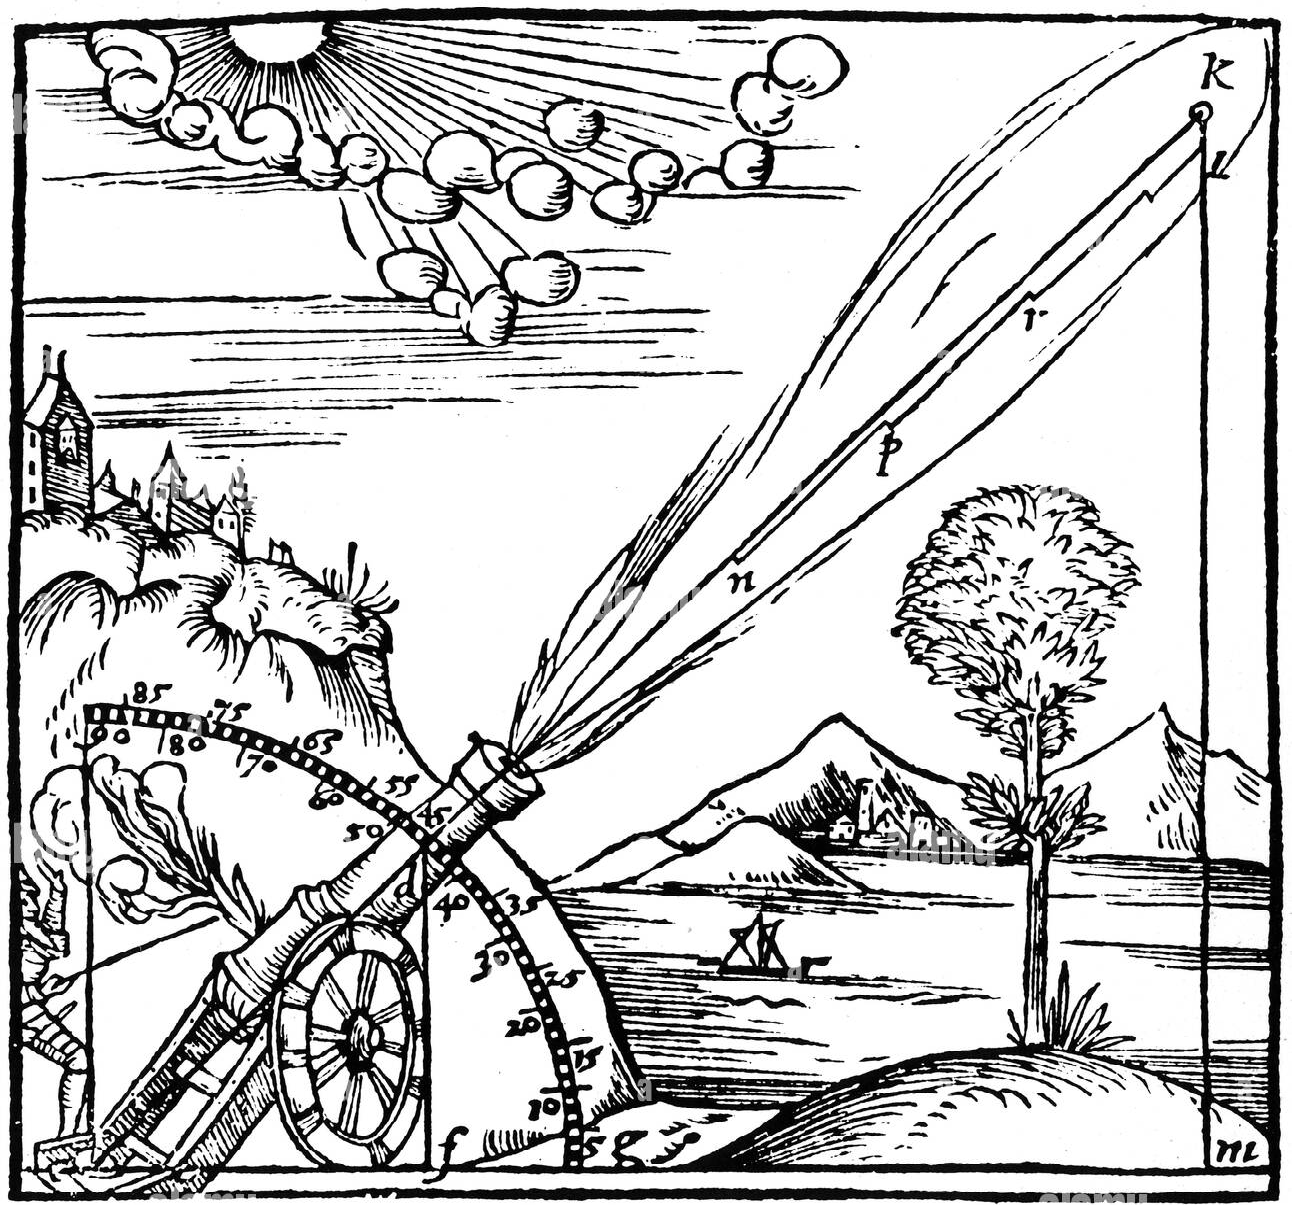
\includegraphics[width=0.75\textwidth]{lanzamiento.png}\par}
\vfill
{\Large Autora: \par}
{\Large Aroa Antón Samaniego \par}
\vfill
{\itshape\Large Mecánica Newtoniana y Relatividad. Prácticas de ordenador.Grado en Física. \par}
{\Large Curso 2022-2023 \par}
\end{titlepage}
    \tableofcontents\hspace{5cm}\pagebreak
\section{Introducción}
Desde la Edad Media se han utilizado cañones en las batallas que se han ido desarrollando y perfeccionando hasta hoy en día. El problema principal que se encontró fue cómo apuntarlos para que el proyectil cayera en el lugar deseado, ya que se han de tener en cuenta muchos factores como la velocidad inicial, el viento, el ángulo, la rotación de la Tierra...\newline\linebreak
En esta práctica vamos a atacar este problema estudiando como afecta la rotación de la Tierra en un tiro parabólico puro.

\section{Cuestiones}
Al tener en cuenta la rotación de la Tierra definimos la aceleración como:
\begin{equation}
\vec{a} = \vec{g} + (\vec{\omega}\times\vec{r})\times\vec{\omega} +2\vec{v}\times\vec{\omega}
\end{equation}
Donde $(\vec{\omega}\times\vec{r})\times\vec{\omega}$ es el término centrípeto y $2\vec{v}\times\vec{\omega}$ es el término de Coriolis.\newline\linebreak
Para ver cómo afectan estas componentes de la aceleración al movimiento, veamos cómo cambia este si anulamos alguna de estas aceleraciones.
\begin{figure}[H]
 \centering
  \subfloat[Con Coriolis y centrípeta]{
   \label{Fig1a}
    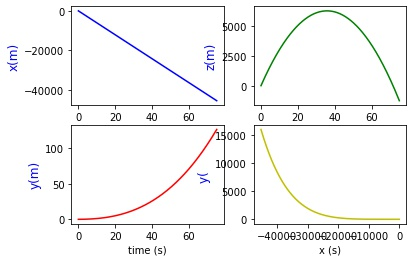
\includegraphics[width=0.5\textwidth]{trayectorias}}
  \subfloat[Sin centrípeta]{
   \label{Fig1b}
    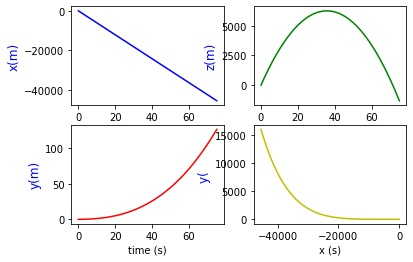
\includegraphics[width=0.5\textwidth]{trayectoriassincentripeta}} 
 \caption{Trayectorias del proyectil}
\label{fig1}
\end{figure}

Como podemos ver en las gráficas, al anular la centrípeta el movimiento sigue siendo prácticamente igual al que tenemos con ambas aceleraciones en juego.
\begin{figure}[H]
 \centering
  \subfloat[Trayectoria sin Coriolis]{
   \label{Fig1a}
    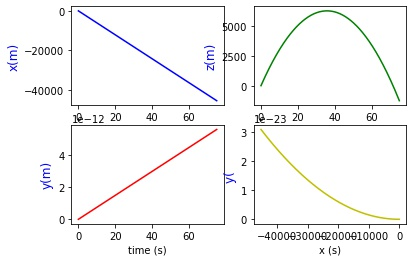
\includegraphics[width=0.5\textwidth]{trayectoriassincoriolis}}
  \subfloat[Trayectoria sin Coriolis en 3D]{
   \label{Fig1b}
    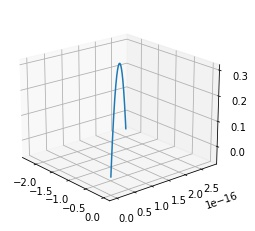
\includegraphics[width=0.4\textwidth]{trayectoriassincoriolis3d}} 
 \caption{Trayectoria del proyectil sin la fuerza de Coriolis}
\label{fig1}
\end{figure}
Sin embargo, si anulamos la fuerza de Coriolis vemos que el tiro se asemeja más al tiro puro. Esto se debe a que la única componente que actúa en la dirección del eje $y$, y que por tanto la modifica, es la fuerza de Coriolis. Por lo que podemos concluir que la fuerza de Coriolis va a jugar un papel más importante que el término centrípeto.\newline\linebreak
Veamos ahora que ocurre si modificamos el ángulo de orientación (la dirección en la que disparamos) del tiro corregido, de tal manera que intentemos que coincida con los resultados del tiro puro.
\begin{figure}[H]
 \centering
  \subfloat[Ángulo aumentado]{
   \label{Fig1a}
    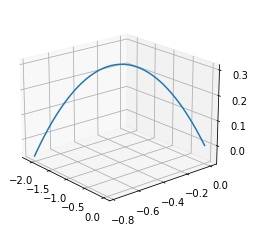
\includegraphics[width=0.3\textwidth]{trayectoria3danguloaumento}}
  \subfloat[180 grados]{
   \label{Fig1b}
    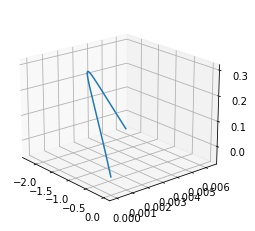
\includegraphics[width=0.3\textwidth]{trayectoria3dangulo}} 
  \subfloat[Ángulo disminuido]{
   \label{Fig1b}
    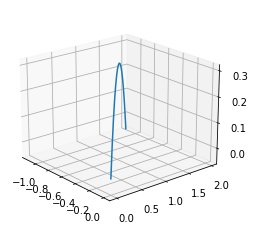
\includegraphics[width=0.3\textwidth]{trayectoria3danguloreducido}}
 \caption{Trayectorias del proyectil para diferentes ángulos de orientación }
\label{fig1}
\end{figure}
\begin{figure}[H]
 \centering
  \subfloat[Ángulo aumentado]{
   \label{Fig1a}
    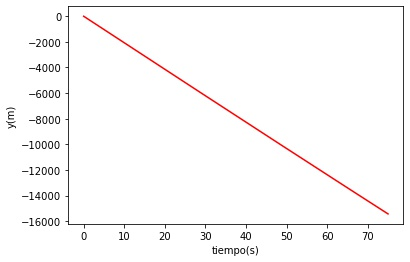
\includegraphics[width=0.3\textwidth]{trayectoriaanguloaumento}}
  \subfloat[180 grados]{
   \label{Fig1b}
    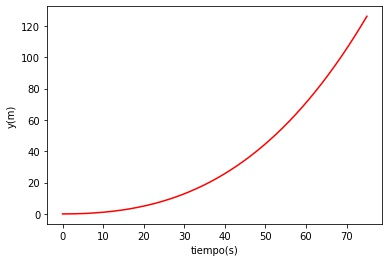
\includegraphics[width=0.3\textwidth]{trayectoriaangulo}} 
  \subfloat[Ángulo disminuido]{
   \label{Fig1b}
    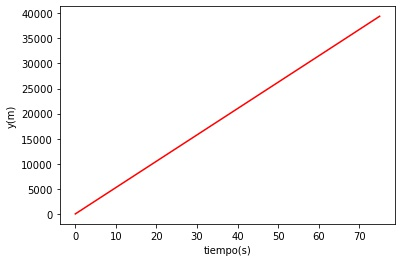
\includegraphics[width=0.3\textwidth]{trayectoriaanguloreducido}}
 \caption{Trayectorias del proyectil para diferentes ángulos de orientación }
\label{fig1}
\end{figure}
Como vemos en las figuras 3 y 4, una pequeña variación en el ángulo provoca grandes cambios en la componente $y$ del tiro. Además, podemos observar que si disminuimos el ángulo la posición $y$ final del tiro aumenta, y si lo aumentamos disminuye.\newline\linebreak
Si vamos probando ángulos para acercarnos lo más posible a la posición final predicha por el tiro puro, tenemos que nos acercamos más en torno a los $180.14^o$. Por lo tanto, si queremos que la posición final de ambos tiros coincida tendríamos que lanzarlos con una diferencia de, aproximadamente, $0.14^o$ , con el ángulo del tiro corregido más grande.\newline\linebreak
Observemos ahora que pasa si modificamos el ángulo de inclinación del tiro.
\begin{figure}[H]
 \centering
   \label{Fig1a}
    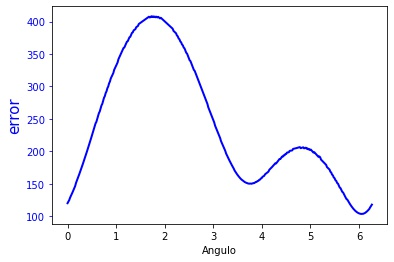
\includegraphics[width=0.5\textwidth]{error}
\end{figure}
A más inclinación el proyectil recorre menos distancia en el eje horizontal y más en el eje vertical, por ello, podemos ver que el error va disminuyendo. Esto se debe a que en las ecuaciones de movimiento del tiro aparece la velocidad inicial, que depende del ángulo de inclinación inicial. Por lo que si aumentamos este también aumentamos la velocidad inicial en el eje vertical.\newline\linebreak
Por último, vamos a ver que pasa si cambiamos la latitud del disparo.
\begin{figure}[H]
 \centering
  \subfloat[Trayectoria latitud positiva]{
   \label{Fig1a}
    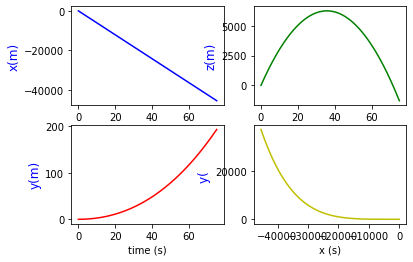
\includegraphics[width=0.5\textwidth]{latitudpositiva}}
  \subfloat[Trayectoria latitud negativa]{
   \label{Fig1b}
    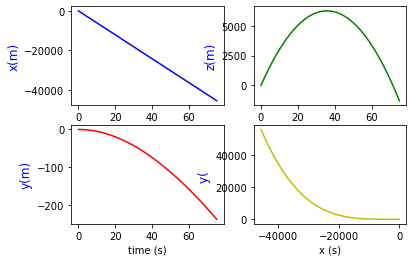
\includegraphics[width=0.5\textwidth]{latitudnegativa}} 
 \caption{Trayectorias del proyectil dependiendo de la latitud}
\label{fig1}
\end{figure}
\begin{figure}[H]
 \centering
  \subfloat[Trayectoria latitud positiva]{
   \label{Fig1a}
    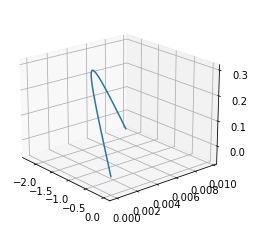
\includegraphics[width=0.4\textwidth]{latitudpositiva3d}}
  \subfloat[Trayectoria latitud negativa]{
   \label{Fig1b}
    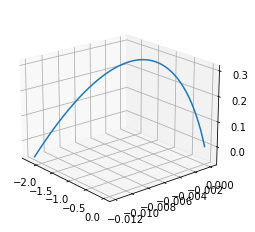
\includegraphics[width=0.4\textwidth]{latitudnegativa3d}} 
 \caption{Trayectorias del proyectil en 3D}
\label{fig1}
\end{figure}
Podemos ver que si modificamos la latitud y nos quedamos en el mismo hemisferio varía la $y$ final, pero conserva el signo. Sin embargo, si nos vamos a latitudes negativas, es decir, disparamos desde el hemisferio sur, la componente $y$ final toma valores negativos. Esto se debe a que la velocidad angular de la Tierra es:
\begin{equation}
\vec{\omega}=\omega(-cos(\phi),0,sen(\phi))
\end{equation}
Donde $\phi$ es la latitud, por lo que al depender la velocidad angular de esta, la aceleración  centrípeta y la fuerza de Coriolis también lo harán,  y al tomar esta valores negativos, los resultados del tiro corregido cambiarán.
\section{Conclusiones}
Hemos podido comprobar como afecta la rotación de la Tierra al lanzamiento de proyectiles. Si observamos todas las modificaciones que hemos ido haciendo como variar los ángulos o la latitud nos damos cuenta que cada vez que variamos un parámetro lo que hacemos es, sobre todo, variar la componente $y$ del tiro, que también es la que modifica principalmente la fuerza de Coriolis y la que se aleja más del tiro puro, por lo que es la que más debemos tener en cuenta si queremos que nuestro proyectil caiga donde predice el tiro puro.
\end{document}